\documentclass{article}

% content/resources/templates/preamble.tex
\usepackage[margin=0.6in]{geometry}
\author{Milav Dabgar}
\usepackage{amsmath,amssymb,amsthm}
\usepackage{booktabs}
\usepackage{multirow}
\usepackage{xcolor}
\usepackage{tcolorbox}
\tcbuselibrary{breakable,skins}
\usepackage[colorlinks=true,linkcolor=blue]{hyperref}
\usepackage{titlesec}
\usepackage{enumitem}
\usepackage{tikz}
\usepackage{pgfplots}
\usepackage{circuitikz}
\usepackage[version=4]{mhchem}
\usepackage{longtable}
\usepackage{array}
\usepackage{float}
\usepackage{caption}
\usepackage{listings}

\lstset{
  basicstyle=\small\ttfamily,
  breaklines=true,
  breakatwhitespace=false,
  postbreak=\mbox{\textcolor{red}{$\hookrightarrow$}\space},
  float=false,
  numbers=left,
  numberstyle=\tiny\color{gray},
  numbersep=10pt,
  xleftmargin=2em,
  keywordstyle=\color{blue},
  commentstyle=\color{green!60!black},
  stringstyle=\color{purple},
  backgroundcolor=\color{gray!5},
  showstringspaces=false,
  tabsize=2,
  captionpos=b,
  keepspaces=true,
  columns=flexible
}

\pgfplotsset{compat=1.18}
\usetikzlibrary{shapes,arrows,positioning,calc,patterns,decorations.pathmorphing,decorations.markings,arrows.meta}

% Color scheme
\definecolor{headcolor}{RGB}{0,102,204}
\definecolor{keycolor}{RGB}{220,20,60}
\definecolor{solutioncolor}{RGB}{34,139,34}
\definecolor{mnemoniccolor}{RGB}{148,0,211}
\definecolor{codecolor}{RGB}{0,0,100}

% Spacing
\setlength{\parskip}{3pt}
\setlist[itemize]{nosep}
\setlist[enumerate]{nosep}

% Title formatting
\titleformat{\section}{\Large\bfseries\color{headcolor}}{\thesection}{1em}{}
\titleformat{\subsection}{\large\bfseries\color{headcolor}}{\thesubsection}{1em}{}

% Pandoc tightlist compatibility
\providecommand{\tightlist}{%
  \setlength{\itemsep}{0pt}\setlength{\parskip}{0pt}}

% Pandoc longtable compatibility
\newcounter{none}
\def\thenone{}


% content/resources/templates/english-boxes.tex

% Custom environments
\newtcolorbox{solutionbox}{
 breakable,
 enhanced,
 colback=solutioncolor!5!white,
 colframe=solutioncolor!75!black,
 fonttitle=\bfseries,
 title=Solution
}

\newtcolorbox{solutionboxnobreak}{
 colback=solutioncolor!5!white,
 colframe=solutioncolor!75!black,
 fonttitle=\bfseries,
 title=Solution
}

\newtcolorbox{keyformula}{
 breakable,
 enhanced,
 colback=keycolor!5!white,
 colframe=keycolor!75!black,
 fonttitle=\bfseries,
 title=Key Formula
}

\newtcolorbox{mnemonicboxenv}{
 breakable,
 enhanced,
 colback=mnemoniccolor!5!white,
 colframe=mnemoniccolor!75!black,
 fonttitle=\bfseries,
 title=Mnemonic
}

\newcommand{\mnemonicbox}[1]{%
  \begin{mnemonicboxenv}
    #1
  \end{mnemonicboxenv}
}


% Custom commands for GTU solutions
% This file defines semantic commands for consistent formatting

% Question command with automatic formatting
\newcommand{\question}[2]{%
  \section*{Question #1}%
  \textbf{#2}%
}

% OR question variant
\newcommand{\questionor}[2]{%
  \section*{Question #1 OR}%
  \textbf{#2}%
}

% Proper table environment with caption
\newenvironment{answertable}[1]{%
  \begin{table}[htbp]
  \centering
  \caption{#1}
}{%
  \end{table}
}

% Proper figure environment for diagrams
\newenvironment{answerdiagram}[1]{%
  \begin{figure}[htbp]
  \centering
  \caption{#1}
}{%
  \end{figure}
}

% Semantic markup for key terms
\newcommand{\keyword}[1]{\textbf{#1}}
\newcommand{\code}[1]{\texttt{#1}}
\newcommand{\classname}[1]{\texttt{#1}}
\newcommand{\methodname}[1]{\texttt{#1}}

% Proper quotation marks
\newcommand{\mnemonic}[1]{``#1''}


\title{Physics (4300005) - Summer 2024 Solution}
\date{June 12, 2024}

\begin{document}
\maketitle

\questionmarks{1(a)}{3}{Define derived physical quantities and give three examples with their S.I. unit and symbol.}

\begin{solutionbox}
Derived physical quantities are those which are obtained by multiplication or division of fundamental physical quantities.

\begin{center}
\captionof{table}{Examples of Derived Physical Quantities}
\begin{tabulary}{\linewidth}{|L|L|L|}
\hline
\textbf{Derived Quantity} & \textbf{S.I. Unit} & \textbf{Symbol} \\ \hline
Force & Newton (N) & F \\ \hline
Energy & Joule (J) & E \\ \hline
Electric Current & Ampere (A) & I \\ \hline
\end{tabulary}
\end{center}
\end{solutionbox}

\begin{mnemonicbox}
\mnemonic{FEI: Force-Energy-Current derive from fundamentals}
\end{mnemonicbox}

\questionmarks{1(b)}{4}{The length of a metal rod is 64.522 cm at 12°C temperature and 64.576 cm at 90°C temperature. Find the coefficient of linear expansion of the metal rod.}

\begin{solutionbox}
\textbf{Formula:} $\alpha = \frac{L_2 - L_1}{L_1 \times (T_2 - T_1)}$

\textbf{Calculation:}
\begin{itemize}
    \item Initial length ($L_1$) = 64.522 cm
    \item Final length ($L_2$) = 64.576 cm
    \item Initial temperature ($T_1$) = 12°C
    \item Final temperature ($T_2$) = 90°C
\end{itemize}

$$
\alpha = \frac{64.576 - 64.522}{64.522 \times (90 - 12)}
$$
$$
\alpha = \frac{0.054}{64.522 \times 78}
$$
$$
\alpha = \frac{0.054}{5032.716}
$$
$$
\alpha = 1.073 \times 10^{-5} /^\circ C
$$
\end{solutionbox}

\begin{mnemonicbox}
\mnemonic{Change in Length over Original Length times Change in Temperature}
\end{mnemonicbox}

\questionmarks{1(c)}{7}{Explain with figure: The principle, construction and working of a vernier calliper.}

\begin{solutionbox}
\textbf{Principle}: Vernier caliper works on the principle of vernier scale, which allows measurements with accuracy greater than the main scale.

\textbf{Construction:}
\begin{center}
\begin{tikzpicture}[node distance=1.5cm, auto]
    \node [gtu block] (V) {Vernier Caliper};
    \node [gtu block, below left=1cm and -1cm of V] (M) {Main Scale};
    \node [gtu block, below right=1cm and -1cm of V] (S) {Vernier Scale};
    \node [gtu block, below=2.5cm of V] (J) {Jaws (Fixed \& Movable)};
    
    \path [gtu arrow] (V) -- (M);
    \path [gtu arrow] (V) -- (S);
    \path [gtu arrow] (V) -- (J);
\end{tikzpicture}
\captionof{figure}{Components of Vernier Caliper}
\end{center}

\textbf{Diagram:}
\begin{center}
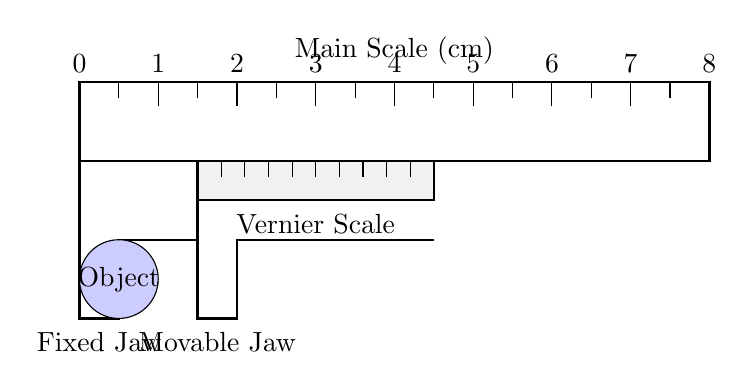
\begin{tikzpicture}
    % Main Scale
    \draw[thick] (0,0) rectangle (8,1);
    \foreach \x in {0,1,...,8} \draw (\x,1) -- (\x,0.7) node[above=3mm] {\x};
    \foreach \x in {0.5,1.5,...,7.5} \draw (\x,1) -- (\x,0.8);
    \node at (4,1.4) {Main Scale (cm)};
    
    % Vernier Scale
    \draw[thick, fill=gray!10] (1.5,-0.5) rectangle (4.5,0);
    \foreach \x in {1.5,1.8,...,4.5} \draw (\x,0) -- (\x,-0.2);
    \node at (3,-0.8) {Vernier Scale};
    
    % Jaws
    \draw[thick] (0,0) -- (0,-2) -- (0.5,-2) -- (0.5,-1) -- (1.5,-1) -- (1.5,0);
    \node at (0.25,-2.3) {Fixed Jaw};
    
    \draw[thick] (1.5,-0.5) -- (1.5,-2) -- (2,-2) -- (2,-1) -- (4.5,-1);
    \node at (1.75,-2.3) {Movable Jaw};
    
    % Object
    \draw[fill=blue!20] (0.5,-1.5) circle (0.5);
    \node at (0.5,-1.5) {Object};
\end{tikzpicture}
\captionof{figure}{Vernier Caliper}
\end{center}

\textbf{Working:}
\begin{itemize}
    \item \textbf{Zero error check}: Close jaws and note if zero of vernier coincides with zero of main scale
    \item \textbf{External measurement}: Place object between fixed and movable jaws
    \item \textbf{Reading process}: Main scale reading + (coinciding vernier division $\times$ least count)
    \item \textbf{Least count} = (Smallest division on main scale)/(Number of divisions on vernier scale)
\end{itemize}
\end{solutionbox}

\begin{mnemonicbox}
\mnemonic{Main Scale Reading Plus Vernier Division Times Least Count}
\end{mnemonicbox}

\questionmarks{1(c OR)}{7}{Explain with figure: The principle, construction and working of a micrometre screw gauge.}

\begin{solutionbox}
\textbf{Principle}: Micrometer screw gauge works on the principle of screw motion - rotational motion is converted into linear motion.

\textbf{Construction:}
\begin{center}
\begin{tikzpicture}[node distance=1.5cm, auto]
    \node [gtu block] (M) {Micrometer};
    \node [gtu block, below left=1cm of M] (F) {Frame};
    \node [gtu block, below=1cm of M] (S) {Spindle \& Anvil};
    \node [gtu block, below right=1cm of M] (T) {Thimble \& Sleeve};
    
    \path [gtu arrow] (M) -- (F);
    \path [gtu arrow] (M) -- (S);
    \path [gtu arrow] (M) -- (T);
\end{tikzpicture}
\captionof{figure}{Components of Micrometer}
\end{center}

\textbf{Diagram:}
\begin{center}
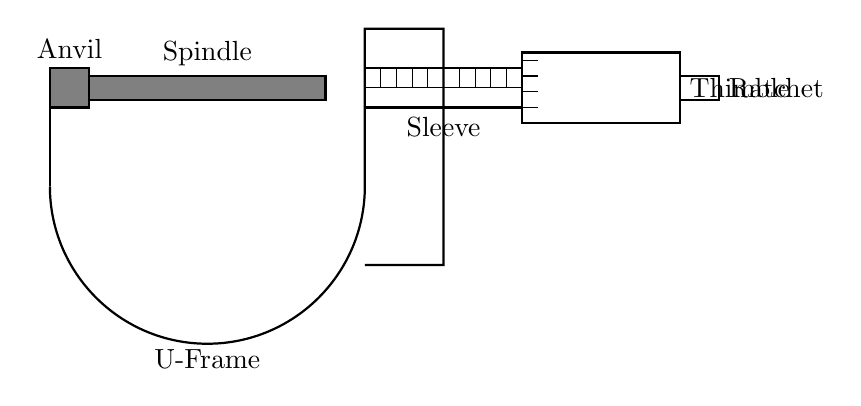
\begin{tikzpicture}
    % Frame
    \draw[thick] (0,0) arc (180:360:2cm) -- (4,0) -- (4,2) -- (5,2) -- (5,-1) -- (4,-1);
    \draw[thick] (0,0) -- (0,1);
    
    % Anvil
    \draw[thick, fill=gray] (0,1) rectangle (0.5,1.5);
    \node[above] at (0.25,1.5) {Anvil};
    
    % Spindle
    \draw[thick, fill=gray] (0.5,1.1) rectangle (3.5,1.4);
    \node[above] at (2,1.4) {Spindle};
    
    % Sleeve
    \draw[thick] (4,1) rectangle (6,1.5);
    \foreach \x in {4,4.2,...,6} \draw (\x,1.25) -- (\x,1.5);
    \draw (4,1.25) -- (6,1.25);
    \node[below] at (5,1) {Sleeve};
    
    % Thimble
    \draw[thick] (6,0.8) rectangle (8,1.7);
    \foreach \y in {0.8,1.0,...,1.7} \draw (6,\y) -- (6.2,\y);
    \node[right] at (8,1.25) {Thimble};
    
    % Ratchet
    \draw[thick] (8,1.1) rectangle (8.5,1.4);
    \node[right] at (8.5,1.25) {Ratchet};
    
    % Frame Label
    \node at (2,-2.2) {U-Frame};
\end{tikzpicture}
\captionof{figure}{Micrometer Screw Gauge}
\end{center}

\textbf{Working:}
\begin{itemize}
    \item \textbf{Zero error check}: Close anvil and spindle, note if zero of circular scale aligns with reference line
    \item \textbf{Measurement process}: Place object between anvil and spindle
    \item \textbf{Reading}: Main scale reading + (Circular scale reading $\times$ Least count)
    \item \textbf{Least Count} = Pitch/Number of divisions on circular scale
\end{itemize}
\end{solutionbox}

\begin{mnemonicbox}
\mnemonic{PST: Pitch divided by Scale gives Thimble's least count}
\end{mnemonicbox}

\questionmarks{2(a)}{3}{Find the diameter of a sphere if pitch of micrometer screw gauge is 1 mm and there are 100 divisions on circular scale. The edge of circular scale lies between 7 and 8 mm of the main scale and 65th division of the circular scale coincides with the horizontal line of the main scale.}

\begin{solutionbox}
\textbf{Formula:} Diameter = Main scale reading + (Circular scale reading $\times$ Least count)

\textbf{Calculation:}
\begin{itemize}
    \item Main scale reading = 7 mm
    \item Circular scale reading = 65 divisions
    \item Least count = Pitch/Number of divisions = 1/100 = 0.01 mm
\end{itemize}

$$
\text{Diameter} = 7 + (65 \times 0.01) = 7 + 0.65 = 7.65 \text{ mm}
$$
\end{solutionbox}

\begin{mnemonicbox}
\mnemonic{MSR + (CSR times LC) gives the final measurement}
\end{mnemonicbox}

\questionmarks{2(b)}{4}{Explain phase difference and coherence.}

\begin{solutionbox}
\textbf{Phase Difference:}
The difference in phase angle between two waves of the same frequency.

\begin{center}
\captionof{table}{Phase Difference Characteristics}
\begin{tabulary}{\linewidth}{|L|L|L|}
\hline
\textbf{Phase Difference} & \textbf{Interference Type} & \textbf{Result} \\ \hline
0° or 360° & Constructive & Maximum amplitude \\ \hline
180° & Destructive & Minimum amplitude \\ \hline
\end{tabulary}
\end{center}

\textbf{Coherence:}
Property of waves that have a constant phase relationship.

\textbf{Types of Coherence:}
\begin{itemize}
    \item \textbf{Temporal coherence}: Related to frequency stability
    \item \textbf{Spatial coherence}: Related to wavefront uniformity
\end{itemize}
\end{solutionbox}

\begin{mnemonicbox}
\mnemonic{Constant Phase Relationship Creates Coherent waves}
\end{mnemonicbox}

\questionmarks{2(c)}{7}{Explain capacitor, its capacitance and the effect of dielectric material on the capacitance of parallel plate capacitor.}

\begin{solutionbox}
\textbf{Capacitor}: Device that stores electric charge and electrical energy in an electric field.

\textbf{Capacitance}: Ratio of charge stored to potential difference applied.

\textbf{Formula:} $C = Q/V$

\textbf{Parallel Plate Capacitor:}
Capacitance formula: $C = \frac{\epsilon_0 A}{d}$
\begin{itemize}
    \item $\epsilon_0$ = Permittivity of free space
    \item $A$ = Area of plates
    \item $d$ = Distance between plates
\end{itemize}

\textbf{Effect of Dielectric:}
\begin{itemize}
    \item Increases capacitance by $K$ times ($K$ = dielectric constant)
    \item New formula: $C = \frac{K \epsilon_0 A}{d}$
\end{itemize}

\textbf{Diagram:}
\begin{center}
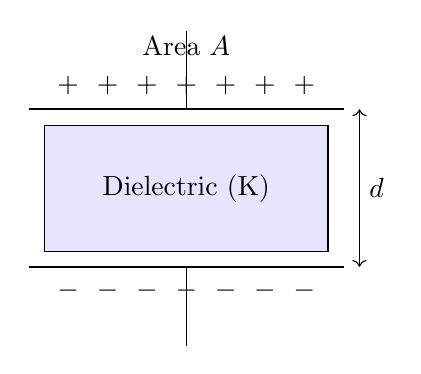
\begin{tikzpicture}
    % Plates
    \draw[thick] (0,2) -- (4,2);
    \draw[thick] (0,0) -- (4,0);
    
    % Charges
    \foreach \x in {0.5,1,...,3.5} \node at (\x,2.3) {$+$};
    \foreach \x in {0.5,1,...,3.5} \node at (\x,-0.3) {$-$};
    
    % Dielectric
    \draw[fill=blue!10] (0.2,0.2) rectangle (3.8,1.8);
    \node at (2,1) {Dielectric (K)};
    
    % Labels
    \draw[<->] (4.2,0) -- (4.2,2) node[midway, right] {$d$};
    \node at (2,2.8) {Area $A$};
    
    % Terminals
    \draw (2,2) -- (2,3);
    \draw (2,0) -- (2,-1);
\end{tikzpicture}
\captionof{figure}{Parallel Plate Capacitor with Dielectric}
\end{center}
\end{solutionbox}

\begin{mnemonicbox}
\mnemonic{KIDS: K Increases Dielectric Storage}
\end{mnemonicbox}

\questionmarks{2(a OR)}{3}{If the lengths of two cylinders are (6.52$\pm$0.01) cm and (4.48$\pm$0.02) cm respectively. Find the difference in their length with percentage error.}

\begin{solutionbox}
\textbf{Calculation:}
\begin{itemize}
    \item Length of first cylinder ($L_1$) = $6.52 \pm 0.01$ cm
    \item Length of second cylinder ($L_2$) = $4.48 \pm 0.02$ cm
    \item Difference in length ($\Delta L$) = $L_1 - L_2 = 6.52 - 4.48 = 2.04$ cm
\end{itemize}

\textbf{Absolute error in difference} = $\sqrt{(0.01)^2 + (0.02)^2} = \sqrt{0.0001 + 0.0004} = \sqrt{0.0005} = 0.022$ cm

\textbf{Percentage error} = $\frac{\text{Absolute error}}{\text{Measured value}} \times 100$
$$
= \frac{0.022}{2.04} \times 100 = 1.08\%
$$
\end{solutionbox}

\begin{mnemonicbox}
\mnemonic{Add errors in quadrature for difference calculations}
\end{mnemonicbox}

\questionmarks{2(b OR)}{4}{Explain the types of interference with relevant figures.}

\begin{solutionbox}
\textbf{Types of Interference:}

\begin{center}
\captionof{table}{Interference Types}
\begin{tabulary}{\linewidth}{|L|L|L|L|}
\hline
\textbf{Type} & \textbf{Phase Difference} & \textbf{Result} & \textbf{Amplitude} \\ \hline
Constructive & 0°, 360°, 720°... & Reinforcement & Maximum \\ \hline
Destructive & 180°, 540°, 900°... & Cancellation & Minimum \\ \hline
\end{tabulary}
\end{center}

\textbf{Constructive Interference:}
When crest meets crest or trough meets trough.

\textbf{Destructive Interference:}
When crest meets trough.

\textbf{Diagram:}
\begin{center}
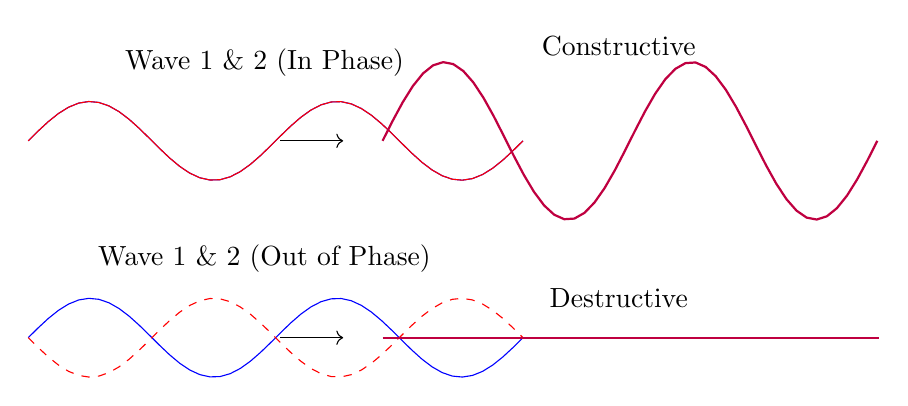
\begin{tikzpicture}
    % Constructive
    \begin{scope}[xshift=0cm]
        \draw[blue] plot[domain=0:4*pi, samples=50] (\x/2, {0.5*sin(\x r)});
        \draw[red] plot[domain=0:4*pi, samples=50] (\x/2, {0.5*sin(\x r)});
        \node at (3,1) {Wave 1 \& 2 (In Phase)};
        
        \draw[->] (3.2,0) -- (4,0);
        
        \draw[purple, thick] plot[domain=0:4*pi, samples=50] (\x/2+4.5, {sin(\x r)});
        \node at (7.5,1.2) {Constructive};
    \end{scope}
    
    % Destructive
    \begin{scope}[yshift=-2.5cm]
        \draw[blue] plot[domain=0:4*pi, samples=50] (\x/2, {0.5*sin(\x r)});
        \draw[red, dashed] plot[domain=0:4*pi, samples=50] (\x/2, {-0.5*sin(\x r)});
        \node at (3,1) {Wave 1 \& 2 (Out of Phase)};
        
        \draw[->] (3.2,0) -- (4,0);
        
        \draw[purple, thick] (4.5,0) -- (10.8,0);
        \node at (7.5,0.5) {Destructive};
    \end{scope}
\end{tikzpicture}
\captionof{figure}{Types of Interference}
\end{center}
\end{solutionbox}

\begin{mnemonicbox}
\mnemonic{Crest + Crest = Constructive, Crest + Trough = Destructive}
\end{mnemonicbox}

\questionmarks{2(c OR)}{7}{Derive the expression for potential due to point charge with necessary figure.}

\begin{solutionbox}
\textbf{Potential at a point due to point charge:}

\textbf{Formula development:}
\begin{itemize}
    \item \textbf{Definition}: Work done per unit charge to bring a test charge from infinity to that point
    \item \textbf{Expression}: $V = W/q_0 = \int (F \cdot dr)$
\end{itemize}

\textbf{Step-by-step derivation:}
\begin{enumerate}
    \item Force between charges (Coulomb's law): $F = \frac{1}{4\pi\epsilon_0} \times \frac{Qq}{r^2}$
    \item Work done moving test charge: $W = \int (F \cdot dr)$
    \item For radial motion: $W = \frac{Q}{4\pi\epsilon_0} \times \int_{\infty}^{r} \frac{1}{r^2} dr$
    \item Integrating: $W = \frac{Q}{4\pi\epsilon_0} \times [-\frac{1}{r}]_{\infty}^{r}$
    \item Final result: $V = \frac{W}{q_0} = \frac{1}{4\pi\epsilon_0} \frac{Q}{r}$
\end{enumerate}

\textbf{Final formula:} $V = \frac{1}{4\pi\epsilon_0} \frac{Q}{r}$

\textbf{Diagram:}
\begin{center}
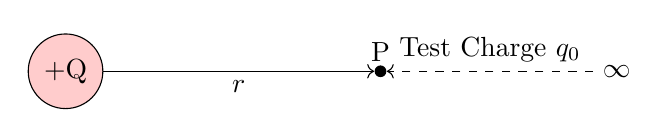
\begin{tikzpicture}
    % Charge Q
    \node[circle, draw, fill=red!20] (Q) at (0,0) {+Q};
    
    % Point P
    \node[circle, fill, inner sep=1.5pt] (P) at (4,0) {};
    \node[above] at (4,0) {P};
    
    % Distance r
    \draw[->] (Q) -- (P) node[midway, below] {$r$};
    
    % Infinity
    \node (Inf) at (7,0) {$\infty$};
    \draw[dashed, ->] (Inf) -- (P) node[midway, above] {Test Charge $q_0$};
\end{tikzpicture}
\captionof{figure}{Potential due to Point Charge}
\end{center}
\end{solutionbox}

\begin{mnemonicbox}
\mnemonic{POD: Potential Over Distance equals charge over r}
\end{mnemonicbox}

\questionmarks{3(a)}{3}{Explain in brief charging by friction and induction methods.}

\begin{solutionbox}
\textbf{Charging by Friction:}
Process of charging by rubbing two different materials together.

\textbf{Steps in friction charging:}
\begin{itemize}
    \item Electrons transfer from one material to another
    \item Material losing electrons becomes positively charged
    \item Material gaining electrons becomes negatively charged
\end{itemize}

\textbf{Charging by Induction:}
Process of charging without direct contact.

\textbf{Steps in induction charging:}
\begin{itemize}
    \item Bring charged body near a neutral conductor
    \item Redistribution of charges in neutral body
    \item Ground the conductor and remove ground
    \item Remove the charged body
\end{itemize}
\end{solutionbox}

\begin{mnemonicbox}
\mnemonic{FTEE: Friction Transfers Electrons Easily}
\end{mnemonicbox}

\questionmarks{3(b)}{4}{A tuning fork vibrates at frequency of 256 Hz. If its velocity is 340 m/s, find (a) wavelength and (b) distance travelled by it in 50 oscillations.}

\begin{solutionbox}
\textbf{Formulas:}
\begin{itemize}
    \item Wavelength ($\lambda$) = Velocity ($v$) / Frequency ($f$)
    \item Distance ($d$) = Number of oscillations ($n$) $\times$ Wavelength ($\lambda$)
\end{itemize}

\textbf{Calculation:}
(a) Wavelength ($\lambda$) = $v/f = 340/256 = 1.328$ m

(b) Distance ($d$) = $n \times \lambda = 50 \times 1.328 = 66.4$ m
\end{solutionbox}

\begin{mnemonicbox}
\mnemonic{VFD: Velocity, Frequency and Distance are connected}
\end{mnemonicbox}

\questionmarks{3(c)}{7}{Write the principle and construction of a bimetallic thermometer with a labelled diagram. Also mention its advantages and disadvantages.}

\begin{solutionbox}
\textbf{Principle}: Different metals expand differently when heated, causing the strip to bend.

\textbf{Construction:}
\begin{center}
\begin{tikzpicture}[node distance=1.5cm, auto]
    \node [gtu block] (B) {Bimetallic Strip};
    \node [gtu block, right=1cm of B] (P) {Pointer};
    \node [gtu block, right=1cm of P] (S) {Scale};
    
    \path [gtu arrow] (B) -- (P);
    \path [gtu arrow] (P) -- (S);
\end{tikzpicture}
\captionof{figure}{Construction Flow}
\end{center}

\textbf{Working:}
\begin{itemize}
    \item Temperature change causes different expansion rates
    \item Bimetallic strip bends toward metal with lower expansion coefficient
    \item Pointer movement indicates temperature
\end{itemize}

\textbf{Diagram:}
\begin{center}
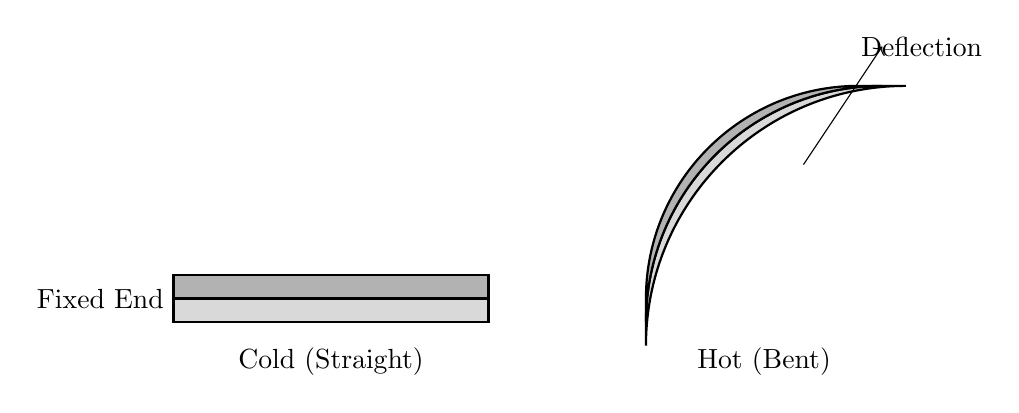
\begin{tikzpicture}
    % Cold State
    \draw[thick, fill=gray!30] (0,0) rectangle (4,0.3);
    \draw[thick, fill=gray!60] (0,0.3) rectangle (4,0.6);
    \node[left] at (0,0.3) {Fixed End};
    \node at (2,-0.5) {Cold (Straight)};
    
    % Hot State
    \begin{scope}[xshift=6cm]
        \draw[thick, fill=gray!30] (0,0) arc (180:90:3cm) -- (3.3,3) arc (90:180:3.3cm) -- cycle;
        \draw[thick, fill=gray!60] (0,0.3) arc (180:90:2.7cm) -- (3,3) arc (90:180:3cm) -- cycle;
        \node at (1.5,-0.5) {Hot (Bent)};
        
        \draw[->] (2,2) -- (3,3.5);
        \node at (3.5,3.5) {Deflection};
    \end{scope}
\end{tikzpicture}
\captionof{figure}{Bimetallic Strip Working}
\end{center}

\textbf{Advantages:}
\begin{itemize}
    \item Simple, robust design
    \item No power supply needed
    \item Wide temperature range
\end{itemize}

\textbf{Disadvantages:}
\begin{itemize}
    \item Less accurate than other types
    \item Slow response time
    \item Subject to mechanical wear
\end{itemize}
\end{solutionbox}

\begin{mnemonicbox}
\mnemonic{BEDS: Bimetallic Elements Deform with Stress}
\end{mnemonicbox}

\questionmarks{3(a OR)}{3}{Explain work done on a point charge in an electric field.}

\begin{solutionbox}
\textbf{Work Done on Point Charge:}
The work done to move a point charge $q$ in an electric field $E$.

\textbf{Formula:}
$$
W = q(V_a - V_{\beta}) = q\Delta V
$$

Where:
\begin{itemize}
    \item $q$ = charge being moved
    \item $V_a$ = potential at initial position
    \item $V_{\beta}$ = potential at final position
    \item $\Delta V$ = potential difference
\end{itemize}

\textbf{Key properties:}
\begin{itemize}
    \item Work is independent of path taken
    \item Work is positive when moving against electric field
    \item Work is negative when moving along electric field
\end{itemize}
\end{solutionbox}

\begin{mnemonicbox}
\mnemonic{PEW: Potential difference times Electric charge equals Work}
\end{mnemonicbox}

\questionmarks{3(b OR)}{4}{What will be the distance travelled by a sound wave in 75 vibrations if its speed is 0.33 km/s and frequency is 660 Hz.}

\begin{solutionbox}
\textbf{Formulas:}
\begin{itemize}
    \item Wavelength ($\lambda$) = Velocity ($v$) / Frequency ($f$)
    \item Distance ($d$) = Number of vibrations ($n$) $\times$ Wavelength ($\lambda$)
\end{itemize}

\textbf{Calculation:}
\begin{itemize}
    \item Convert velocity: $v = 0.33 \text{ km/s} = 330 \text{ m/s}$
    \item Wavelength: $\lambda = v/f = 330/660 = 0.5 \text{ m}$
    \item Distance: $d = n \times \lambda = 75 \times 0.5 = 37.5 \text{ m}$
\end{itemize}
\end{solutionbox}

\begin{mnemonicbox}
\mnemonic{FVW: Frequency into Velocity gives Wavelength}
\end{mnemonicbox}

\questionmarks{3(c OR)}{7}{Write the principle and construction of a Mercury thermometer with a labelled diagram. Also mention its advantages and disadvantages.}

\begin{solutionbox}
\textbf{Principle}: Mercury thermometer works on the principle of thermal expansion of mercury when heated.

\textbf{Construction:}
\begin{center}
\begin{tikzpicture}[node distance=1.5cm, auto]
    \node [gtu block] (B) {Bulb};
    \node [gtu block, right=1cm of B] (C) {Capillary};
    \node [gtu block, right=1cm of C] (V) {Vacuum};
    
    \path [gtu arrow] (B) -- (C);
    \path [gtu arrow] (C) -- (V);
\end{tikzpicture}
\captionof{figure}{Construction Components}
\end{center}

\textbf{Diagram:}
\begin{center}
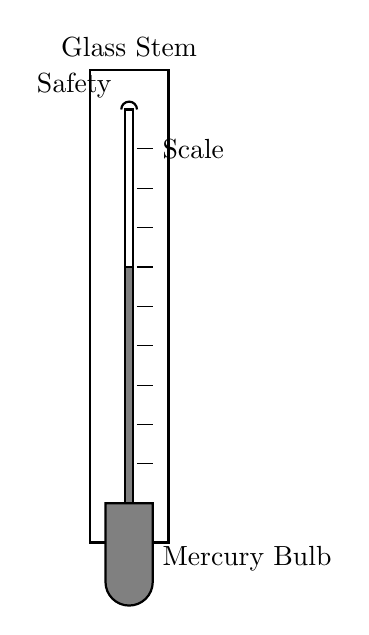
\begin{tikzpicture}
    % Glass Stem
    \draw[thick] (0,0) rectangle (1,6);
    \node at (0.5,6.3) {Glass Stem};
    
    % Capillary
    \draw[thick] (0.45,0.5) rectangle (0.55,5.5);
    \draw[fill=gray] (0.45,0.5) rectangle (0.55,3.5); % Mercury column
    
    % Bulb
    \draw[thick, fill=gray] (0.2,-0.5) arc (180:360:0.3cm) -- (0.8,0.5) -- (0.2,0.5) -- cycle;
    \node[right] at (0.8,-0.2) {Mercury Bulb};
    
    % Scale
    \foreach \y in {1,1.5,...,5} \draw (0.6,\y) -- (0.8,\y);
    \node[right] at (0.8,5) {Scale};
    
    % Safety Bulb
    \draw[thick] (0.4,5.5) arc (180:0:0.1cm);
    \node[left] at (0.4,5.8) {Safety};
\end{tikzpicture}
\captionof{figure}{Mercury Thermometer}
\end{center}

\textbf{Working:}
\begin{itemize}
    \item Mercury expands when heated
    \item Expansion causes mercury to rise in capillary
    \item Height of mercury column indicates temperature
\end{itemize}

\textbf{Advantages:}
\begin{itemize}
    \item High accuracy
    \item Wide temperature range (-38°C to 357°C)
    \item Linear expansion of mercury
    \item Good visibility of mercury thread
\end{itemize}

\textbf{Disadvantages:}
\begin{itemize}
    \item Mercury is toxic
    \item Fragile glass construction
    \item Cannot be used below -38°C
    \item Slow response to temperature changes
\end{itemize}
\end{solutionbox}

\begin{mnemonicbox}
\mnemonic{MELT: Mercury Expands Linearly with Temperature}
\end{mnemonicbox}

\questionmarks{4(a)}{3}{The electric force between two positive ions of equal magnitude separated by distance $5 \times 10^{-10}$ m from eachother is $3.7 \times 10^{-9}$ N. How many electrons would have been removed from each atom.}

\begin{solutionbox}
\textbf{Formula:} $F = \frac{1}{4\pi\epsilon_0} \times \frac{q_1q_2}{r^2}$

\textbf{Calculation:}
\begin{itemize}
    \item $F = 3.7 \times 10^{-9}$ N
    \item $r = 5 \times 10^{-10}$ m
    \item $q_1 = q_2 = ne$ ($n$ = number of electrons, $e$ = electron charge)
    \item $1/4\pi\epsilon_0 = 9 \times 10^9 \text{ Nm}^2/\text{C}^2$
    \item $e = 1.6 \times 10^{-19}$ C
\end{itemize}

$$
3.7 \times 10^{-9} = (9 \times 10^9) \times \frac{n^2 e^2}{(5 \times 10^{-10})^2}
$$
$$
3.7 \times 10^{-9} = (9 \times 10^9) \times \frac{n^2 \times (1.6 \times 10^{-19})^2}{25 \times 10^{-20}}
$$
Solving: $n = 1$ (1 electron removed from each atom)
\end{solutionbox}

\begin{mnemonicbox}
\mnemonic{FACE: Force Affects Charge Equally}
\end{mnemonicbox}

\questionmarks{4(b)}{4}{State Snell's law and derive its formula.}

\begin{solutionbox}
\textbf{Snell's Law}: The ratio of sine of angle of incidence to sine of angle of refraction is constant for a given pair of media.

\textbf{Formula:}
$$
\frac{\sin i}{\sin r} = \frac{n_2}{n_1} = \text{constant}
$$

\textbf{Derivation steps:}
\begin{enumerate}
    \item Light travels at different speeds in different media
    \item When light passes from one medium to another, it changes direction
    \item Using Fermat's principle of least time
    \item Ratio of speeds equals ratio of refractive indices
    \item Final formula: $n_1 \sin i = n_2 \sin r$
\end{enumerate}

\textbf{Diagram:}
\begin{center}
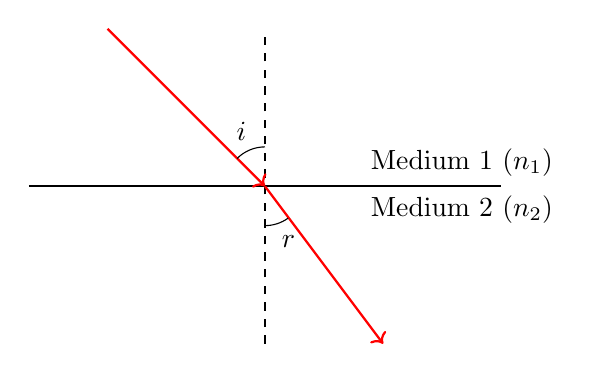
\begin{tikzpicture}
    % Interface
    \draw[thick] (-3,0) -- (3,0);
    \node[above] at (2.5,0) {Medium 1 ($n_1$)};
    \node[below] at (2.5,0) {Medium 2 ($n_2$)};
    
    % Normal
    \draw[dashed] (0,-2) -- (0,2);
    
    % Rays
    \draw[red, thick, ->] (-2,2) -- (0,0);
    \draw[red, thick, ->] (0,0) -- (1.5,-2);
    
    % Angles
    \draw (0,0.5) arc (90:135:0.5);
    \node at (-0.3,0.7) {$i$};
    
    \draw (0,-0.5) arc (270:306:0.5);
    \node at (0.3,-0.7) {$r$};
\end{tikzpicture}
\captionof{figure}{Refraction and Snell's Law}
\end{center}
\end{solutionbox}

\begin{mnemonicbox}
\mnemonic{SINIS: SIN I over SIN R equals refractive index ratio}
\end{mnemonicbox}

\questionmarks{4(c)}{7}{Explain any three applications of Ultrasonic waves.}

\begin{solutionbox}
\textbf{Applications of Ultrasonic Waves:}

\begin{center}
\captionof{table}{Ultrasonic Applications}
\begin{tabulary}{\linewidth}{|L|L|L|}
\hline
\textbf{Application} & \textbf{Principle} & \textbf{Use} \\ \hline
Medical Imaging & Reflection from tissues & Visualize internal organs \\ \hline
NDT (Non-Destructive Testing) & Reflection from defects & Find flaws in materials \\ \hline
Cleaning & Cavitation effect & Clean jewelry, surgical instruments \\ \hline
\end{tabulary}
\end{center}

\textbf{1. Medical Imaging (Sonography):}
\begin{itemize}
    \item Frequencies: 1-10 MHz
    \item Principle: Pulse-echo technique
    \item Uses: Fetal imaging, organ scanning, blood flow measurement
\end{itemize}

\textbf{2. Industrial NDT:}
\begin{itemize}
    \item Detects cracks, voids, and flaws in materials
    \item Quality control in manufacturing
    \item Thickness measurement of materials
\end{itemize}

\textbf{3. Ultrasonic Cleaning:}
\begin{itemize}
    \item Creates microscopic bubbles (cavitation)
    \item Removes contaminants from surfaces
    \item Used for jewelry, optical components, surgical instruments
\end{itemize}
\end{solutionbox}

\begin{mnemonicbox}
\mnemonic{MIC: Medical, Industrial, Cleaning applications}
\end{mnemonicbox}

\questionmarks{4(a OR)}{3}{Obtain the equivalent capacitance for series and parallel combinations of 3 capacitors having capacitances 5 $\mu$F, 10 $\mu$F and 15 $\mu$F respectively.}

\begin{solutionbox}
\textbf{Parallel Combination:}
$$
C_p = C_1 + C_2 + C_3 = 5 + 10 + 15 = 30 \mu F
$$

\textbf{Series Combination:}
$$
\frac{1}{C_s} = \frac{1}{C_1} + \frac{1}{C_2} + \frac{1}{C_3}
$$
$$
\frac{1}{C_s} = \frac{1}{5} + \frac{1}{10} + \frac{1}{15}
$$
$$
\frac{1}{C_s} = 0.2 + 0.1 + 0.067 = 0.367
$$
$$
C_s = \frac{1}{0.367} = 2.72 \mu F
$$
\end{solutionbox}

\begin{mnemonicbox}
\mnemonic{ASAP: Add for Series, Add inverse for Parallel}
\end{mnemonicbox}

\questionmarks{4(b OR)}{4}{Explain the construction of an optical fibre with a neat diagram.}

\begin{solutionbox}
\textbf{Construction of Optical Fiber:}

\textbf{Components:}
\begin{itemize}
    \item Core: Light transmission medium
    \item Cladding: Outer layer with lower refractive index
    \item Buffer coating: Protective plastic covering
\end{itemize}

\textbf{Parameters:}
\begin{itemize}
    \item Core diameter: 8-50 $\mu$m (single mode), 50-100 $\mu$m (multimode)
    \item Cladding diameter: 125-140 $\mu$m
    \item Core refractive index $>$ Cladding refractive index
\end{itemize}

\textbf{Diagram:}
\begin{center}
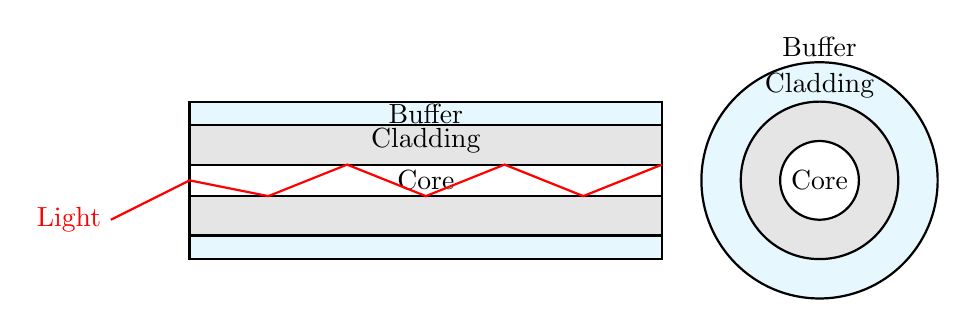
\begin{tikzpicture}
    % Longitudinal view
    \draw[thick, fill=cyan!10] (0,0) rectangle (6,2); % Buffer
    \draw[thick, fill=gray!20] (0,0.3) rectangle (6,1.7); % Cladding
    \draw[thick, fill=white] (0,0.8) rectangle (6,1.2); % Core
    
    \node at (3,1) {Core};
    \node at (3,1.5) {Cladding};
    \node at (3,1.85) {Buffer};
    
    % Light Ray
    \draw[red, thick] (-1,0.5) -- (0,1) -- (1,0.8) -- (2,1.2) -- (3,0.8) -- (4,1.2) -- (5,0.8) -- (6,1.2);
    \node[red, left] at (-1,0.5) {Light};
    
    % Cross Section
    \begin{scope}[xshift=8cm, yshift=1cm]
        \draw[thick, fill=cyan!10] (0,0) circle (1.5);
        \draw[thick, fill=gray!20] (0,0) circle (1);
        \draw[thick, fill=white] (0,0) circle (0.5);
        
        \node at (0,0) {Core};
        \node at (0,1.2) {Cladding};
        \node at (0,1.7) {Buffer};
    \end{scope}
\end{tikzpicture}
\captionof{figure}{Optical Fiber Construction}
\end{center}
\end{solutionbox}

\begin{mnemonicbox}
\mnemonic{CBC: Core-Buffer-Cladding from inside out}
\end{mnemonicbox}

\questionmarks{4(c OR)}{7}{Explain production of ultrasonic waves by magnetostriction method.}

\begin{solutionbox}
\textbf{Magnetostriction Method:}
The process of generating ultrasonic waves using the property of ferromagnetic materials to change dimensions when placed in a magnetic field.

\textbf{Principle:}
Ferromagnetic materials change length when magnetized, producing mechanical vibrations that create ultrasonic waves.

\textbf{Construction:}
\begin{center}
\begin{tikzpicture}[node distance=1.5cm, auto]
    \node [gtu block] (P) {AC Power};
    \node [gtu block, below=1cm of P] (C) {Coil/Solenoid};
    \node [gtu block, below=1cm of C] (R) {Ferro. Rod};
    \node [gtu block, right=1cm of R] (U) {Ultrasonic Waves};
    
    \path [gtu arrow] (P) -- (C);
    \path [gtu arrow] (C) -- (R);
    \path [gtu arrow] (R) -- (U);
\end{tikzpicture}
\captionof{figure}{Magnetostriction Process}
\end{center}

\textbf{Working Process:}
\begin{enumerate}
    \item AC current passes through solenoid
    \item Alternating magnetic field produced
    \item Ferromagnetic rod expands and contracts
    \item Vibrations transmitted to medium
    \item Ultrasonic waves generated
\end{enumerate}

\textbf{Diagram:}
\begin{center}
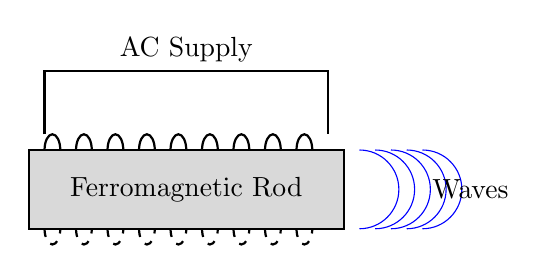
\begin{tikzpicture}
    % Rod
    \draw[thick, fill=gray!30] (2,0) rectangle (6,1);
    \node at (4,0.5) {Ferromagnetic Rod};
    
    % Coil
    \foreach \x in {2.2,2.6,...,5.8} \draw[thick] (\x,1) arc (180:0:0.1cm and 0.2cm);
    \foreach \x in {2.2,2.6,...,5.8} \draw[thick, dashed] (\x,0) arc (180:360:0.1cm and 0.2cm);
    \draw[thick] (2.2,1.2) -- (2.2,2) -- (5.8,2) -- (5.8,1.2);
    \node[above] at (4,2) {AC Supply};
    
    % Waves
    \foreach \x in {6.2,6.4,...,7.0} \draw[blue] (\x,0) arc (-90:90:0.5);
    \node[right] at (7,0.5) {Waves};
\end{tikzpicture}
\captionof{figure}{Magnetostriction Oscillation}
\end{center}

\textbf{Advantages:}
\begin{itemize}
    \item Simple construction
    \item High power output
    \item Suitable for liquids
\end{itemize}

\textbf{Disadvantages:}
\begin{itemize}
    \item Limited to frequencies below 100 kHz
    \item Heating effects
    \item Lower efficiency
\end{itemize}
\end{solutionbox}

\begin{mnemonicbox}
\mnemonic{FAME: Ferromagnetic Alternating Magnetic Effect}
\end{mnemonicbox}

\questionmarks{5(a)}{3}{Explain in brief the three modes of heat transfer.}

\begin{solutionbox}
\textbf{Three Modes of Heat Transfer:}

\begin{center}
\captionof{table}{Heat Transfer Modes}
\begin{tabulary}{\linewidth}{|L|L|L|}
\hline
\textbf{Mode} & \textbf{Medium Requirement} & \textbf{Example} \\ \hline
Conduction & Physical contact & Heat through metal rod \\ \hline
Convection & Fluid medium & Hot air rising \\ \hline
Radiation & No medium needed & Heat from sun \\ \hline
\end{tabulary}
\end{center}

\begin{enumerate}
    \item \textbf{Conduction:}
    \begin{itemize}
        \item Transfer through direct molecular collision
        \item No bulk movement of matter
        \item Good in solids, especially metals
    \end{itemize}
    
    \item \textbf{Convection:}
    \begin{itemize}
        \item Transfer through fluid movement
        \item Requires density differences
        \item Natural or forced convection
    \end{itemize}
    
    \item \textbf{Radiation:}
    \begin{itemize}
        \item Transfer through electromagnetic waves
        \item Works in vacuum
        \item Depends on temperature and surface properties
    \end{itemize}
\end{enumerate}
\end{solutionbox}

\begin{mnemonicbox}
\mnemonic{CCR: Conduction Contact, Convection Current, Radiation Rays}
\end{mnemonicbox}

\questionmarks{5(b)}{4}{Calculate the numerical aperture and acceptance angle of an optical fibre if the refractive indices of core and cladding of an optical fibre are 1.55 and 1.5 respectively.}

\begin{solutionbox}
\textbf{Formulas:}
\begin{itemize}
    \item Numerical Aperture (NA) = $\sqrt{n_1^2 - n_2^2}$
    \item Acceptance angle ($\theta_a$) = $\sin^{-1}(\text{NA})$
\end{itemize}

\textbf{Calculation:}
\begin{itemize}
    \item Core refractive index ($n_1$) = 1.55
    \item Cladding refractive index ($n_2$) = 1.5
\end{itemize}

$$
\text{NA} = \sqrt{1.55^2 - 1.5^2} = \sqrt{2.4025 - 2.25} = \sqrt{0.1525} = 0.391
$$

$$
\theta_a = \sin^{-1}(0.391) = 23.03^\circ
$$
\end{solutionbox}

\begin{mnemonicbox}
\mnemonic{CORE: Calculate Optical Refractive-index Exactly}
\end{mnemonicbox}

\questionmarks{5(c)}{7}{Explain any three applications of optical fibres.}

\begin{solutionbox}
\textbf{Applications of Optical Fibers:}

\begin{center}
\captionof{table}{Major Optical Fiber Applications}
\begin{tabulary}{\linewidth}{|L|L|L|}
\hline
\textbf{Application} & \textbf{Advantage} & \textbf{Example} \\ \hline
Communications & High bandwidth & Internet, phone networks \\ \hline
Medical & Flexibility, imaging & Endoscopy \\ \hline
Sensors & Immunity to EMI & Temperature sensing \\ \hline
\end{tabulary}
\end{center}

\textbf{1. Communication Networks:}
\begin{itemize}
    \item Telecommunications and internet
    \item Higher bandwidth than copper cables
    \item Less signal attenuation over long distances
\end{itemize}

\textbf{2. Medical Applications:}
\begin{itemize}
    \item Endoscopy for minimally invasive procedures
    \item Light delivery for photodynamic therapy
    \item Surgical illumination
\end{itemize}

\textbf{3. Sensing Applications:}
\begin{itemize}
    \item Temperature and pressure sensors
    \item Strain gauges for structural monitoring
    \item Gyroscopes for navigation
\end{itemize}
\end{solutionbox}

\begin{mnemonicbox}
\mnemonic{CMS: Communication, Medical, Sensing applications}
\end{mnemonicbox}

\questionmarks{5(a OR)}{3}{Give a detailed explanation of specific heat.}

\begin{solutionbox}
\textbf{Specific Heat:}
Amount of heat required to raise the temperature of 1 kg of a substance by 1 Kelvin (or 1°C).

\textbf{Formula:} $Q = mc\Delta T$

Where:
\begin{itemize}
    \item $Q$ = Heat energy (J)
    \item $m$ = Mass (kg)
    \item $c$ = Specific heat capacity (J/kg·K)
    \item $\Delta T$ = Temperature change (K)
\end{itemize}

\textbf{Units:} J/kg·K or J/kg·°C

\textbf{Significance:}
\begin{itemize}
    \item Measures thermal inertia of materials
    \item Higher specific heat means material requires more energy to heat up
    \item Water has unusually high specific heat (4,186 J/kg·K)
\end{itemize}
\end{solutionbox}

\begin{mnemonicbox}
\mnemonic{STEM: Specific heat measures Temperature change per Energy and Mass}
\end{mnemonicbox}

\questionmarks{5(b OR)}{4}{If the refractive indices of core and cladding of an optical fibre are 1.48 and 1.45 respectively. Calculate its acceptance angle and critical angle.}

\begin{solutionbox}
\textbf{Formulas:}
\begin{itemize}
    \item Numerical Aperture (NA) = $\sqrt{n_1^2 - n_2^2}$
    \item Acceptance angle ($\theta_a$) = $\sin^{-1}(\text{NA})$
    \item Critical angle ($\theta_c$) = $\sin^{-1}(n_2/n_1)$
\end{itemize}

\textbf{Calculation:}
\begin{itemize}
    \item Core refractive index ($n_1$) = 1.48
    \item Cladding refractive index ($n_2$) = 1.45
\end{itemize}

$$
\text{NA} = \sqrt{1.48^2 - 1.45^2} = \sqrt{2.1904 - 2.1025} = \sqrt{0.0879} = 0.296
$$
$$
\theta_a = \sin^{-1}(0.296) = 17.2^\circ
$$
$$
\theta_c = \sin^{-1}(1.45/1.48) = \sin^{-1}(0.9797) = 78.4^\circ
$$
\end{solutionbox}

\begin{mnemonicbox}
\mnemonic{NA leads to AA, ratio leads to Critical Angle}
\end{mnemonicbox}

\questionmarks{5(c OR)}{7}{Explain the applications of LASER in engineering and medical field.}

\begin{solutionbox}
\textbf{Applications of LASER:}

\begin{center}
\captionof{table}{LASER Applications}
\begin{tabulary}{\linewidth}{|L|L|L|}
\hline
\textbf{Field} & \textbf{Application} & \textbf{Example} \\ \hline
Engineering & Cutting/Welding & Metal fabrication \\ \hline
Engineering & Measurements & Distance measurement \\ \hline
Medical & Surgery & Eye surgery (LASIK) \\ \hline
Medical & Therapy & Cancer treatment \\ \hline
\end{tabulary}
\end{center}

\textbf{Engineering Applications:}
\begin{enumerate}
    \item \textbf{Material Processing:}
    \begin{itemize}
        \item Precision cutting of metals, plastics, ceramics
        \item Welding of dissimilar materials
        \item 3D printing and rapid prototyping
    \end{itemize}
    
    \item \textbf{Metrology and Measurement:}
    \begin{itemize}
        \item Distance measurement with high precision
        \item Alignment in construction and manufacturing
        \item Holography for 3D imaging
    \end{itemize}
\end{enumerate}

\textbf{Medical Applications:}
\begin{enumerate}
    \item \textbf{Surgical Procedures:}
    \begin{itemize}
        \item Eye surgery (LASIK, cataract removal)
        \item Minimally invasive procedures
        \item Dental procedures
    \end{itemize}
    
    \item \textbf{Therapeutic Uses:}
    \begin{itemize}
        \item Photodynamic therapy for cancer
        \item Low-level laser therapy for pain
        \item Cosmetic procedures
    \end{itemize}
\end{enumerate}

\textbf{Diagram:}
\begin{center}
\begin{tikzpicture}[node distance=1.5cm, auto]
    \node [gtu block] (L) {LASER};
    \node [gtu block, below left=1.5cm of L] (E) {Engineering};
    \node [gtu block, below right=1.5cm of L] (M) {Medical};
    
    \path [gtu arrow] (L) -- (E);
    \path [gtu arrow] (L) -- (M);
    
    \node [gtu block, below=0.5cm of E] (E1) {Cutting/Welding};
    \node [gtu block, below=0.5cm of M] (M1) {Surgery/Therapy};
    
    \path [gtu arrow] (E) -- (E1);
    \path [gtu arrow] (M) -- (M1);
\end{tikzpicture}
\captionof{figure}{Fields of Laser Application}
\end{center}
\end{solutionbox}

\begin{mnemonicbox}
\mnemonic{SMART: Surgery, Measurement, Analysis, Repair, and Treatment}
\end{mnemonicbox}

\end{document}
